\documentclass[12pt]{article}
\usepackage[utf8]{inputenc}
\usepackage{xcolor}
\usepackage{graphicx}
\usepackage{listings}
\usepackage{epstopdf}
\usepackage{etoc}
\usepackage{pdfpages}
\usepackage[capposition=top]{floatrow}
\usepackage{pdflscape} % landsacpe package
% set font to times
%\usepackage{mathptmx} % times!!! 
%\usepackage[T1]{fontenc}
\usepackage{amsmath}
\usepackage{soul}
\usepackage[left=2.5cm, right=2.5cm, top=2.5cm, bottom =2.5cm]{geometry}
\usepackage[round, authoryear]{natbib}
%\usepackage[natbibapa]{apacite}
%\usepackage{apacite}
%\bibliographystyle{apacite}
\bibliographystyle{plainnat} % to see all authors' names
%\renewcommand{\footnotesize}{\fontsize{10pt}{11pt}\selectfont}
\usepackage[onehalfspacing]{setspace}
\usepackage{listings}
\renewcommand{\figurename}{\textbf{Figure}}
\renewcommand{\hat}{\widehat}
\usepackage[bf]{caption}
\usepackage{tikz}
%\begin{comment}
%\usepackage[headsepline,footsepline]{scrlayer-scrpage} % has to come before package!!! otherwise option clash
%\usepackage{scrlayer-scrpage}
%\pagestyle{scrheadings} % kopfzeile/ fußzeile
%\clearpairofpagestyles
%\ohead{}
%\ihead{\textit{Redistribution, Demand and  Sustainable Production}}
%\cfoot{\thepage}
%\pagestyle{plain} % comment this one to have header
%\end{comment}
\usepackage{comment}
 \usepackage{siunitx}
  \usepackage{textcomp}
\definecolor{sonja}{cmyk}{0.9,0,0.3,0}
%\definecolor{purple}{model}{color-spec}
\usepackage{amssymb}
\newcommand{\ar}{$\Rightarrow$ \ }
\newcommand{\frp}[2]{\frac{\partial{#1}}{\partial{#2}}}
\newcommand{\tr}[1]{\textcolor{red}{#1}}
\newcommand{\vlt}[1]{\textcolor{violet}{#1}}
\newcommand{\bl}[1]{\textcolor{blue}{#1}}
\newcommand{\sn}[1]{\textcolor{sonja}{#1}}
%%% TIKZS
\usepackage{tikz}
%\usepackage{times}
\usetikzlibrary{mindmap,trees}
\usetikzlibrary{backgrounds}
\tikzstyle{every edge}=  [fill=orange]  
\usetikzlibrary{tikzmark}
\usetikzlibrary{decorations.markings}
\usepackage{tikz-cd}
\usetikzlibrary{arrows,calc,fit}
\tikzset{mainbox/.style={draw=sonja, text=black, fill=white, ellipse, rounded corners, thick, node distance=5em, text width=8em, text centered, minimum height=3.5em}}
\tikzset{mainboxbig/.style={draw=sonja, text=black, fill=white, ellipse, rounded corners, thick, node distance=5em, text width=13em, text centered, minimum height=3.5em}}
\tikzset{dummybox/.style={draw=none, text=black , rectangle, rounded corners, thick, node distance=4em, text width=20em, text centered, minimum height=3.5em}}
\tikzset{box/.style={draw , rectangle, rounded corners, thick, node distance=7em, text width=8em, text centered, minimum height=3.5em}}
\tikzset{container/.style={draw, rectangle, dashed, inner sep=2em}}
\tikzset{line/.style={draw, very thick, -latex'}}
\tikzset{    pil/.style={
		->,
		thick,
		shorten <=2pt,
		shorten >=2pt,}}
	
% other stuff
\newcommand{\innermid}{\nonscript\;\delimsize\vert\nonscript\;}
\newcommand{\activatebar}{%
	\begingroup\lccode`\~=`\|
	\lowercase{\endgroup\let~}\innermid 
	\mathcode`|=\string"8000
}
%\usepackage{biblatex}
%\addbibresource{bib_mt.bib}
\usepackage{ulem}
\title{Related Literature}
\date{Sonja Dobkowitz\\ Bonn Graduate School of Economics\\ %University of Bonn\\
\vspace{1mm}
%Preliminary and incomplete\\
First version: December 21, 2021\\
This version: \today }
\usepackage{graphicx,caption}
\usepackage{hyperref}
\usepackage{minitoc}
\setcounter{secttocdepth}{5}
\usetikzlibrary{shapes.geometric}

% for tabular

%\usepackage{array}
\usepackage{makecell}
\usepackage{multirow}
\usepackage{bigdelim}

\renewenvironment{abstract}
{\small
	\list{}{
		\setlength{\leftmargin}{0.025\textwidth}%
		\setlength{\rightmargin}{\leftmargin}%
	}%
	\item\relax}
{\endlist}
\begin{document}
%	\includepdf[pages=-]{../titlepage.pdf}
	\maketitle
	\tableofcontents
\section{Timeline}
\begin{itemize}
	\item what fields are connected to my research \ar Mindmap \checkmark
	\item literature review to all of them MACRO (environmental is too particular)
	\item read papers broadly
\end{itemize}

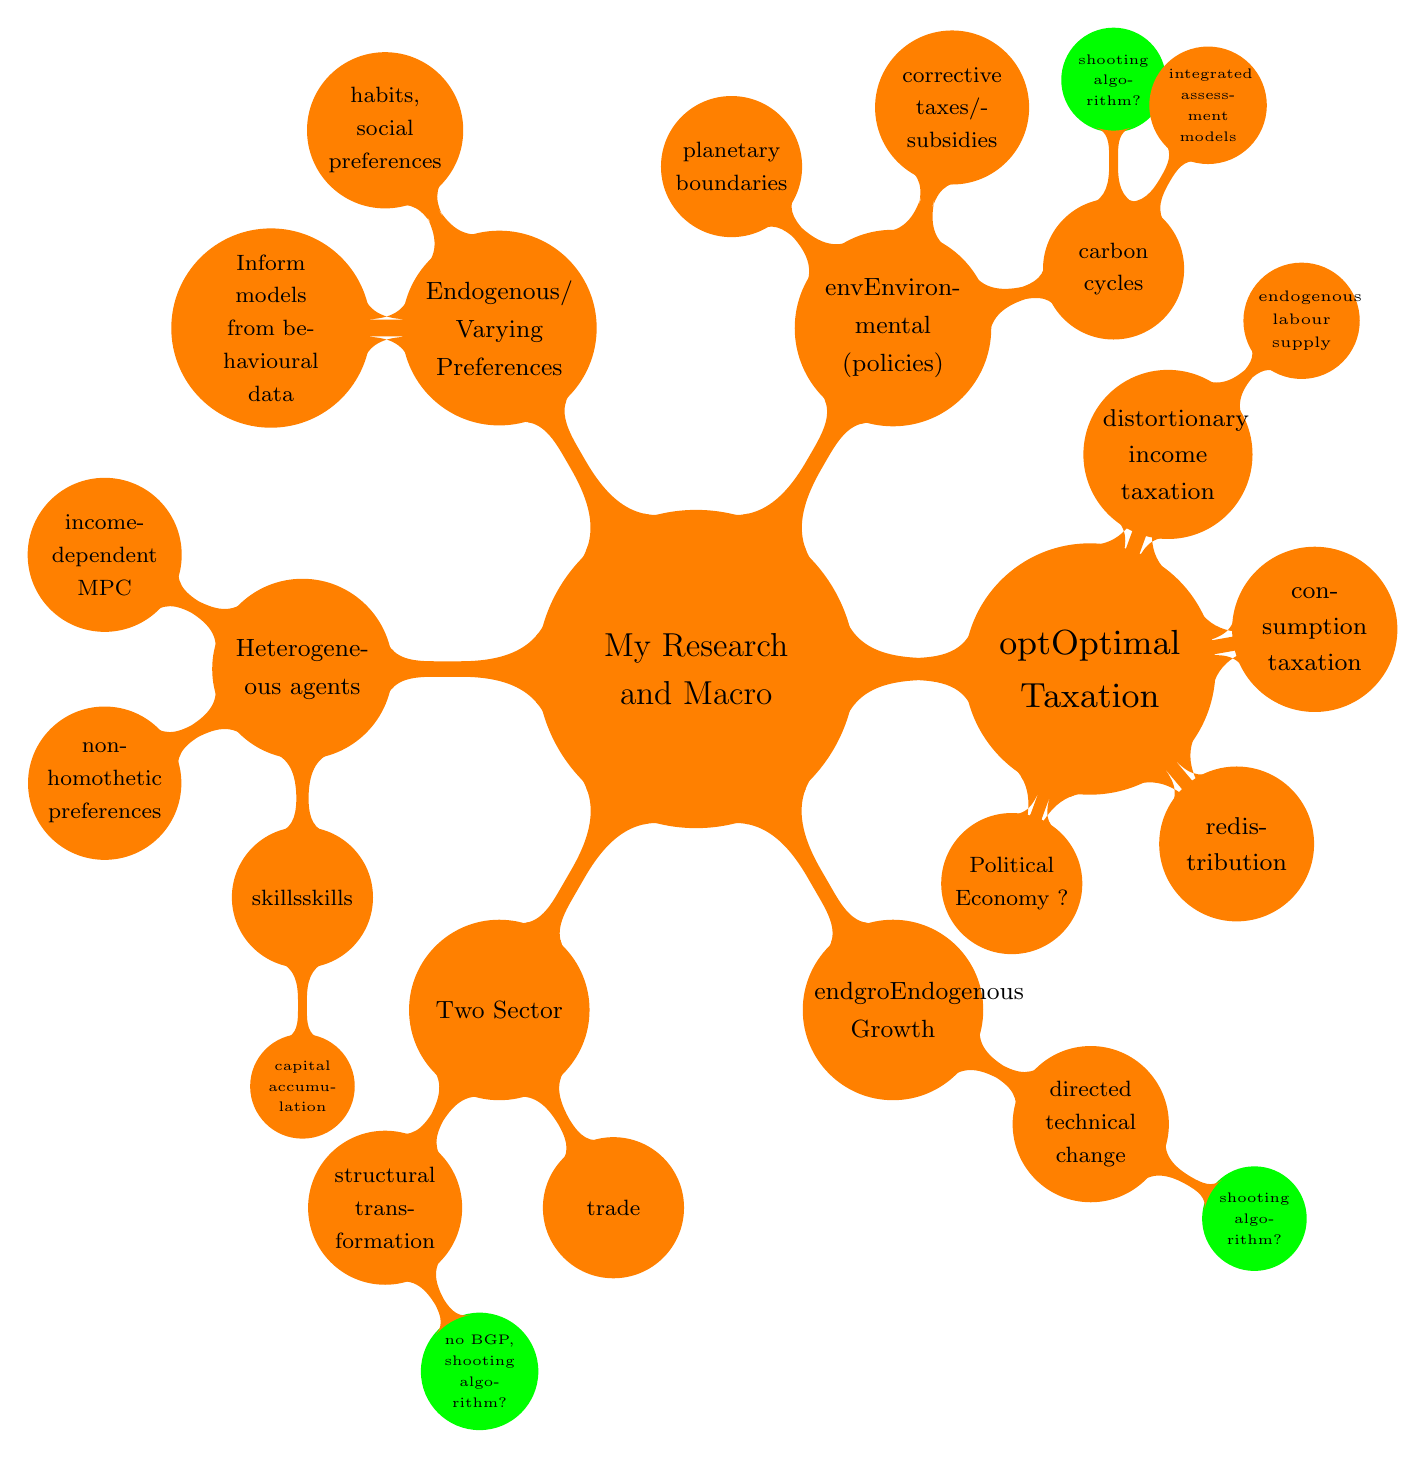
\begin{tikzpicture}[]
\path[mindmap,concept color=orange,text=black]
node[concept] {My Research and Macro}
[clockwise from=0]
child[] {
	node[concept, scale=1.4] {\hyperlink{opt}{Optimal Taxation}}
	[clockwise from=70]
	child { node[concept, scale=1.1] (income tax)  {distortionary income taxation} 
		[clockwise from=45] 
		child { node[concept, scale=1.1] (endLab)  {endogenous labour supply} }}
	child { node[concept, scale=1.1] (cons tax)  {con- sumption taxation} 
%		[clockwise from=90]
%		child {node[concept] {}}
%		child {node[concept, level distance=2cm] {}}
	}
	child { node[concept, scale=1.1] (redist)  {redis- tribution} }	
	child[concept color=orange] { node[concept] {Political Economy ?} 
	}
}	  
child[concept color=orange] {
	node[concept] (endg) {\hyperlink{endgro}{Endogenous Growth}}
	[clockwise from=-30]
	child { node[concept] (dtc) {directed technical change}
			child { node[concept, color=green, text=black] (sh) {shooting algorithm?}
		}  
	}
}
child[concept color=orange] { node[concept] {Two Sector}
		[clockwise from=-60]  
		child { node[concept] (trade) {trade}} 
		child { node[concept] (trans) {structural trans- formation}
			child { node[concept, color=green, text=black] (sh) {no BGP, shooting algorithm?}
		}	
	}
}
child[concept color=orange] { node[concept] {Heterogene- ous agents} 
		[clockwise from=-90]
		child { node[concept] (hetskill) {\hyperlink{skills}{skills}} 
			child { node[concept]  {capital accumulation}}} 
		child { node[concept] (nhp) {non-homothetic preferences}} 
		child { node[concept] (mpc) {income-dependent MPC}} 
}
child[concept color=orange] { node[concept] {Endogenous/ Varying Preferences} 
	[clockwise from=180]
	child { node[concept] (emp) {Inform models from behavioural data}} 
	child { node[concept] (habs) {habits, social preferences}} 
}
child[concept color=orange] { node[concept] {\hyperlink{env}{Environ- mental (policies)}} 
		[clockwise from=135] 
		child { node[concept] (pb) {planetary boundaries}}
	child { node[concept] (corr) {corrective taxes/subsidies}}
	child { node[concept] (cc) {carbon cycles}
		[clockwise from=90] 
		child { node[concept, color=green, text=black] (sh) {shooting algorithm?}
		}
	child { node[concept] (IAM) {integrated assessment models}
	}
	}
}
;

\begin{pgfonlayer}{background}
\draw [circle connection bar ]
;
\end{pgfonlayer}

\end{tikzpicture}

\section{What is there in all papers that my project should not lack?} \ar based on this question decide on what aspect of project to focus on; i.e.,
a project which is connected to optimal taxation, environmental policy/ climate change

\begin{itemize}
	\item $\underline{\textbf{optimal environmental policy}}$
	\begin{itemize}

\item \textbf{endogenous growth} \cite{Hassler2016EnvironmentalMacroeconomics, Acemoglu2016TransitionTechnology, Fried2018ClimateAnalysis};
frequently abstract from capital, savings decision
\item \textbf{carbon cycle} in optimal policy and transition papers \cite{Acemoglu2016TransitionTechnology, Barrage2019OptimalPolicy, Hassler2016EnvironmentalMacroeconomics, Golosov2014OptimalEquilibrium}; \ar I think a carbon cycle alone falls short of the other planetary boundaries as in \cite{Rockstrom2009AHumanity} \ar \textbf{extend carbon cycle for other cycles as a contribution?}
\item \textbf{transitions?} \cite{Acemoglu2016TransitionTechnology, Fried2018ClimateAnalysis}
\item \textbf{focus on energy or two sectors}?\ar two sectors as I will argue that it is not only the energy source (most relevant for carbon) but others two 
\item[\ar] \textbf{What is missing that I could add: }
\begin{itemize}
	\item focus on a broader set of planetary boundaries; carbon free might be available but what about externalities in general? (7/01/22); but then not possible to take exogenously specified policy targets!
\item inequality\ar especially as a determinant of environmental policy functioning
\item distortionary taxes as policy tool not passive
\item uncertainty in environmental boundaries and carbon cycle
\item uncertainty of substitutability of technologies
\item exogenous climate target as in \cite{Fried2018ClimateAnalysis}; but not about optimal policy given carbon targets as a constraint; Advantages: 
\begin{itemize}
\item less prone to uncertainty in parameter values, structure of interaction nature and economy
\end{itemize}
\item changes in household behaviour
\end{itemize}
 
	\end{itemize}

\item $\underline{\textbf{optimal taxation}}$: \ar exogenous revenue target of government, or redistribution, then \ar \textbf{heterogeneous agent} setting.
\begin{itemize}
	\item heterogeneous agents
	\item transitions
\end{itemize}
\end{itemize}

\section{Handbooks}
Of interest:
\begin{itemize}
\item handbook of macroeconomics
\item handbook of endogenous growth
\item handbook of social choice and welfare
\item handbook of computational ecoonomics: heterogeneous agent modelling 
\end{itemize}
\section{Otimal Policy (and Heterogeneity)}
\hypertarget{opt}{}
\localtableofcontents

\subsection{What are reoccurring issues in this field?}\ar \underline{quantitative} optimal taxation \ar optimal distortionary taxation:
\begin{itemize}
	\item skill heterogeneity 
	\item (transitions)
	\item idiosyncratic income risk \ar insurance motive for redistribution
	\item prominent zero capital tax finding
	\item optimal progressivity of labour income tax code
	\item is consumption tax preferable to labour income tax? In literature (see Domeji/Heathcote) large welfare gains switching from labour to consumption taxes/ rep agent
\end{itemize}


\subsection{ \citet*{Heathcote2017OptimalFramework}}

\begin{itemize}
\item a static model when skill´ is instantaneously reversible! 
\item focus on progressivity of labour taxation
\item incorporate skill formation!: 1) in first version: fully reversible skill investment at any time (no transition, plus: no tendency of gov to tax skill as if irreversible)... 2nd slow adjustment in skills implies transitional dynamics
\item heterogeneity in skills and in preferences(!) for work
\item trade-off: (a) equity and insurance against idiosyncratic income risks (pro progressivity) vs. (b) progressivity reduces work incentives and $\underline{to invest in skills}$, plus financing of gov income calls for regressive tax system as the higher work effort allows to increase the tax base (pro regressivity)
\item[\ar] \textcolor{sonja}{Public good could be environmental quality? subsidies to clean sector; investing in skills is depressed by progressivity \ar costly for high-skill sectors; tax has an impact on the extensive margin of a skill and not the intensive margin (hours supplied) in this model }
\item Structure
\begin{enumerate}
\item analytics to qualitatively inspect the distinct channels
\item relative importance assessed quantitatively (when yyy is bigger then xxx and zzz etc... then this and this channel is more important \ar quantitative analysis helpful)
\item compare optimal progressivity to observed progressivity in the US
\item How to square discrepancy? US tax system is more progressive than optimal in terms of the model... eg due to a higher disutility from inequality
\item political economy framework to assess optimal progressivity \ar planner would choose higher progressivity than the utilitarian planner; closer to the US counterpart
\item[\ar] \textcolor{sonja}{Why could progressivity be good in my model? Bcs the rich consume more, this should be reduced}
\item extensions to baseline in form of frictions to skill investment: 
\begin{itemize}
\item skill choice cannot respond to tax reform
\item poverty trap: poor cannot acquire skills
\end{itemize}
\item positive analysis: can theory account for cross-country differences in tax progressivity? i.e. progressivity falls with gov. purchases and rises with inequality
\end{enumerate}
\item Tax Function
\begin{itemize}
\item they use $T(y)=y-\lambda y^{1-\tau}$ as tax revenues; $\lambda y^{1-\tau}$ is hence disposable income
\item their definition of progressivity: if the ratio of \textbf{marginal} to \textbf{average} \textbf{disposable income} is smaller than 1 for all income levels \ar average disposable income is falling with income:
$\frac{1-T'(y)}{1-\frac{T(y)}{y}}=1-\tau$\ar $\tau<0$ then the tax system is regressive, $\tau=0$ flat, the average income tax paid is constant with y (namely $1-\lambda$). With $\tau>0$ the system is progressive
\item $\lambda$ shifts the level of tax revenues, the higher the bigger disposable income
\item break-even income level; $y^0=\lambda^\frac{1}{\tau}$: the disposable income is zero
\item also captures transfers; can become negative
\item statutory rates: tax rate established by the law
\item effective rates: percent of income paid as tax
\end{itemize}
\item Model
\begin{itemize}
	\item Life cycle; perpetual youth structure \ar there is no retirement, each period is the same once skill level has been chosen; survival probability is constant over life cycle
	\item continuum of skill types
	\item skill only input to production; the scarcer a skill level the higher its price due to the imperfect substitutability of skills in the production function $\theta<\infty$ where $\theta$ is the elasticity of substitution
	\item disutility from initial investment into skill (investment differs by skill and household type)
	\item preferences over consumption, hours worked, public good
	\item idiosyncratic productivity shocks
	\item skill investment is endogenous depending on tax system 
	\item competitive markets
	\item government budget: gov chooses spending and progressivity, the level $\lambda$ asjusts to balance the budget (\textit{Is the level irrelevant for HH choices? No under logarithmic utility!})
	\item split period problem into sequential smaller problems (timing of shock realisations, market openings etc. not jointly chosen)
\end{itemize}
	\item \textbf{Rep agent as a special case to full model}:
	\begin{itemize}
	\item all hh have equal tastes for leisure and labour productivity
	\item all skill levels are perfect substitutes (by assumption) \ar no investment into skills
	\end{itemize}
\item recursive formulation of model
\begin{itemize}
\item for each sub-period there is a different state vector and problem
\end{itemize}
\item derive closed-form solution to individual hh problem is relation to Rep agent solution
\begin{itemize}
	\item hours are fixed under a flat tax (rep.agent) and logarithimc, separable utility function! see p.1709\textcolor{sonja}{ \ar same as in my model with flat tax without transfers\ar employ more flexible tax system which can then be solved analytically!}
	\item discuss components of each aspect (use logs! to have a sum)/summand that affects equilibrium hours and consumption \ar in policy function; there is no time subscript as the problem is time invariant due to  the perpetual youth structure
\end{itemize}
\item \textcolor{sonja}{their distributions are continuous instead discrete which would be more helpful if the model was only meant to be solved numerically}
\item private labour supply is inefficiently low as more work would imply higher provision of the public good which gives positive utility; but taken as given 
\item choosing the right pareto weights (weights of individuum in social welfare function) can replicate the competitive equilibrium. Agents with a higher consumption in the competitive equilibrium would need a high pareto weight, with equal weights the planner would redistribute due to concave utility functions to those with lower consumption (p.1715). \ar \tr{Pareto weights are a way to abstract from inequality concerns in social objective function }
\item p.1712:  skill supply is decreasing in progressivity as the premium is reduced
\item the wage of a given skill increases in the skill! This results from: the higher skills the scarcer the number of households with these skills (as less households are willing to invest as much \ar heterogeneity in disutility from skill investment and its distribution)
\item establish concavity of SWF in gov. choice variables to only look at first order conditions
\end{itemize}
\subsection{ \cite{Piketty2013OptimalTaxation} (Handbook of Public Economics)}
\begin{itemize}
\item  Questions to the text 
\begin{itemize}
	\item empirical evidence on labour elasticity/ efficiency channel
	\item what are the motives for labour taxation prominent in the (political) discussion? \ar is there a role for environmental considerations considered somewhere?
	\item What are labour taxes used to?
\end{itemize}
\item issue of welfare function! \ar Idea: compare optimal labour tax with externality to optimal tax resulting from Rawlsian welfare function without externality \ar are they similar?
How do optimal taxes from Utilitarian versus Rawlsian social planner differ?
\item \textbf{Summary Intro, Section 1}
\begin{itemize}
	\item linear taxation
	\item non-linear taxes
	\item median voter tax equilibria
	\item means-tested transfers
	\item rent-seeking models \ar pay differs from productivity
	\item tagging\ar conditioning taxes/ transfers on characteristics correlated with ability 
	\item \textbf{differntial commodity taxation to supplement income tax}\ar does this connect to my paper with reduction policies?
	\item welfarism= how to choose weights on individual utilities
	\item They argue for the following conditions on methods in public finance; optimal policy discussion: (1) based on empirically relevant economic mechanisms, (2) robust to preferences, (3) implementability of tax policy\ar simple (e.g. linear)
\end{itemize}
\item \textbf{Summary section 2: Tax Systems in history and reality}
\begin{itemize}
\item + economic literature; p.403: behavioural in public finance
\item most important findings in theoretical literature:
\begin{itemize}
\item optimal income taxation started with MIrrlees 1971: max social welfare based on individual utilities, behavioural responses of labour supply; people differ wrt skills but gov can only observe earnings \ar equite-efficiency trade-off (if could observe skill could impose 2nd WFT)
\item Result: zero marginal tax at the top earnings level (one more unit of income no more taxes) (Sadka 1976, Seade 1977)
\item  result II: if the minimum earnings level is positive with no bunching of individuals at the bottom \ar marginal tax rate at the bottom is also zero (Seade 1977)
\item result3: Mirrlees (1971), Seade (1982) if redistribution should be from high to low earners, then the marginal tax rate is never negative
\item Stiglitz 1982 discrete version of Mirrlees with two types
\item \ar incentive compatibility constraints on high types not to mimic low types, 
\item Atkinson/Siglitz (1976) under separability and homogeneity of preferences: differentiated commodity taxation is not useful when earnings can be taxed nonlinearly, \ar practical motive for eliminating preferential taxation of necessities on redistributive grounds and instead uniform value-added tax combined with income based transfers and progressive income tax; also used to argue against capital income taxation! and in favour of earnings or consumption taxes
\item Diamond 1980: optimal tax with extensive margin\ar optimal marginal tax rate can then be negative 
\item Saez 2002a: negative marginal rate optimal at the bottom in an extenisve labour supply model 
\end{itemize}
\item elasticities as sufficient statistics
\end{itemize}
\item \textbf{Summary section 3: Conceptual Background}
\begin{itemize}
\item utilitarian social welfare Objective \ar gov. chooses disposable income of each household
\item exogenous pre-tax income distribution \ar Result: full redistribution (no cost to redistribution plus concave utility); differences in utility functions not observable \ar assume homogeneous marginal utility of consumption given income (otherwise enjoying consumption more becomes a motive for redistribution)\ar as if everyone could use resources in a way similar in benefits
\item homogeneous utility functions  with fixed earnings \ar existence of a universal social utility function (based on individual income but same for all), concavity of which determines preference for redistribution, 
\item endogenous labour supply p.405 (\textit{no empirical evidence at this point!})
\item introduce generalised social welfare function $G()$ so that $SWF=\int_0^\infty \omega_i G(u^i(c,z))d\nu(i)$ with $\omega_i$ weight on individual i's utility, $z$ pre-tax earnings, $\nu(i)$ distribution of individuals 
\item \textit{social marginal welfare weights}: $g_i=\frac{\omega_iG'(u^i)u^i_c}{\rho}$ where $\rho$ is the lagrange multiplier on governmental revenues, i.e. the value of public funds \ar From optimality it follows that $g_i$ \textbf{is the price the government is willing to pay for a marginal increase in individual i's consumption at the optimal allocation }
\item with endogenous earnings $g_i's$ are not equalized
\item Rawls: $g_i=0$ for all individuals except the most disadvantaged; Utilitatrian $g_i=\frac{u^i_c}{\rho}$
\item \tr{\textbf{Quasi-linear preferences \ar no income effect!} \textit{This means that the level of transfers does not change behaviour! As does the wage rate through the income effect.. only substitution effect present!}}; \\
Quasi-linear preferences: $u^i(c,z)= v^i(c-h^i(z))$ with $v^i$ increasing and concave, and $h^i$ increasing and convex \ar labour decision does not depend on non-labour income! \ar the average of $g_i$ over all individuals equals 1, since at the optimum the government is indifferent between one more dollar of revenue (with a value of $\rho$) and redistributing one more unit to everyone ($\int_{0}^{\infty}\omega_iG'(u^i)u^i_cd\nu(i)$) (since there are no additional cost through redistribution in terms of efficiency! )
\item[\ar] for my project: In order to disentangle redistributional concerns from efficiency benefit through externality: look at model with quasi-linear preferences and give unlimited resources to government; \tr{\textbf{similar to allow for labour tax but no transfers?\ar the only value of labour tax is to reduce consumption and labour supply \ar simple model to show effect of distortionary tax; in this setup compare effect of policy on externality without endogenous innovation, without heterogeneity}}
\item \textbf{Section 3.2: Fallacy of the 2nd Welfare theorem:} in theory, using information on skills, should be able to implement efficient allocation by use of the 2nd welfare theorem (perfect market assumption: any pareto efficient outcome can be reached through a suitable set of lump-sum transfers which depend on exogenous characteristics of individual)
\item but not done in practice; 1 argument: skills not observed, however, other variables related with skills are neither used, 
\item other explanation: non-standard tax instruments harder to implement
\item or, they ask,  some other aspect of justice that leads to this? \ar Sonja: would force people with high skills to work more in order to pay their taxes; but that seems unfair too... with imperfect markets there is unemployment, 2nd welfare theorem fails with no perfect insurance...
\item \textbf{section 3.3 Labour supply concepst}
\begin{itemize}
\item intensive labour margin \ar characterised by un- and compensated elasticity of labour wrt wage, substitution and income effect. 
\item extensive margin: fixed cost of work, decision on whether to work or not to work. Discrete cost of d when choosinz $z>0$ as opposed to z=0
\item \tr{In model Keith's topics class: there was an extensive labour margin only: work vs not working. If work, than supply all labour}
\end{itemize}
\end{itemize}
\item \textbf{Still to read: chapter 4 \textit{optimal linear taxation}, 5 \textit{optimal nonlinear taxation}, 6 \textit{extensions}}
\item \textbf{Section 7: Alternatives to Welfarist Approach (= Utilitarian ) }
\begin{itemize}
\item Pareto weights\ar weighted sum of utilities; Pareto Principle\ar sub-optimal tax systems: no pareto improvement is left undone
\item Rawlsian Criterion: maxi-min: optimum independent on cardinal choice for individual utilities; need to decide on who is most disadvantaged?
\item libertarianism, benefits principle: no redistribution! 
\item principles of responsibility and Compensation: compensation for circumstances not under control of the individual; responsible for things under control
\item equal opportunity: locally Rawlsian: correct for differences in earnings in the same earnings percentile...
\end{itemize}
\item Supplementary Commodity Taxation p.446
\begin{itemize}
	\item should not be nonlinear due to retrading
	\item value added taxes, general sales taxes
	\item exemption of goods on redistributive grounds
	\item extra taxes on specific goods such as tobacco, alcohol, airplane tickets, motor vehicles \ar excise taxes where traditionally put on goods which were easy to monitor for the government; nowadays due to externalities, 
\end{itemize}
\end{itemize}
\subsection{\cite{Conesa2009TaxingAll}: Conesa, Kitao, Krueger
} \textcolor{sonja}{seems a bit complicated to me. I think I prefer simpler models to highlight one mechanism and then see how the mechanism spells out in a quantitative model}\\
\tr{They find relative to the status quo benchmark a reduction in aggregate consumption and hours worked due to distributional benefits (insurance and equity)}
\begin{itemize}
\item general finding in literature: zero capital tax in long run
\item two modelling choices yield a different finding: (a) uninsurable income risk; (b) life-cycle models
\item[\ar] missing: quantitative determination of optimal capital and labour tax in a realistically calibrated life-cycle model with borrowing contraints and idiosyncratic risk; bcs both elements make positive capital tax possibly optimal
\item highlight role of whether a progressive labour tax tool is available for the optimal capital tax
\item welfare measure: veil of ignorance: ex-ante realization of ability and expected shock process
\item motive for redistribution: (1) heterogeneous ability , (2) insurance against idiosyncratic shocks
\item can be achieved through both capital tax (as higher wealth implies less prone to idiosyncratic labour income risk) or the progressive labour income tax
\item trade-off: insurance and redistribution versus capital or labour distortions
\item findings: capital tax of 36\%, flat labour income tax of 23\% with a deduction of \$7,200; \\
intuition: (1) in life-cycle model optimal to base labour tax on \textbf{age}; here not in policy tool set\ar progressive labour income tax or capital tax both achieve the same!;  (2) costly to tax labour income of the young too heavily due to tight borrowing constraints and upward sloping life-cycle earnings profile. Again, capital tax or progressive labour tax help here
\item there is no transition but there is population growth 
\item Quantitative experiments to find out about the drivers of the results: sequentially adding stuff to a stripped down version of the benchmark model
\begin{itemize}
\item differences in labour supply over the life-cycle drives high capital income tax result
\item market incompleteness and distributional concerns shape progressivity of labour tax
\end{itemize}
\item they cite a bunch of quantitative papers on positive effetcs of tax reforms and on normative tax questions
\item \textit{anonymity} of tax code\ar cannot tax individuum-specific
\item constant capital tax rate = proportional tax= flat tax: $T_k(y_k)=\tau_ky_k$
\item labour income tax are an arbitrary function of taxable labour income: $T(y_t)$; potentially progressive
\item Functional forms: Income tax function $T^{GS}(y)= \kappa_0(y-(y^{-\kappa_1}+\kappa_2)^{\frac{1}{\kappa_1}})$; has been used in the \textbf{quantitative public fincnance} literature previously; 
$\kappa_0$\ar level of the average tax rate; $\kappa_1$\ar determines progressivity; $\kappa_1\rightarrow0$ flat tax code; $\kappa_2$ adjusts to meet government budget purposes; 
\item the tax code parameters are chosen optimally by the government, and $\kappa_2$ residually to meet budget
\item \textbf{Results}: \textit{in this section they show results but also discuss why the allocation,life-cycle profiles are as obeserved} 
\begin{itemize}
\item present results: the optimal tax system
\item  comparison to benchmark (parameters which best approximate US tax system; status quo); Differences in allocation and why
\item welfare: \textbf{optimal tax system features lower aggregate consumption at a modest decline in hours worked}; yet welfare substantially higher. Measured by a consumption equivalent with labour unchanged. \\
Welfare decomposition into labour and consumption changes (consumption divided further into distributional change and aggregate change)\\
\tr{less hours worked\ar smoothes leisure over the life cycle! Better in terms of utility!}
\item allocaton over the life cycle: asset oldings highest between 40-70 (age)\ar decline in assets on aggregate and for every age
\item labour supply reduces when young and increases when old (shortly before retirement)
\item also compare results to empirical findings
\end{itemize}
\item Interpretation and Sensitivity\\ \textit{What is driving the results, ie. the optimal tax code \ar sequentially shut down channels of full model}
\begin{itemize}
\item Main findings: significantly postive capital tax and progressive income tax due to high deduction
\item identify crucial modeling choices/ parameters: 
\begin{itemize}
\item endogenous labour supply \ar labour supply elasticity
\item  borrowing constraints
\item ex-ante heterogeneity in labour productivity
\item idiosyncratic income risk (Markov chain of labour productivity)
\item life-cycle elements: social security, idiosyncratic mortality risk, age-specific element of productivity 
\end{itemize}
\item in a table they compare optimal policies with some features shut 
\item this gives a new set of results but they are meant to see the reasons for why the optimal tax in the benchmark model is as it is
\item findings
\begin{itemize}
\item \textbf{endogenous labour supply drives the positive capital tax rate! }(distortionary aspect)
\item \textbf{with endogenous labour supply the level of the optimal capital tax depends on the life-cycle elements of the model age-specific element of wages/ mortality risk/ social security}
\item borrowing constraints and idiosyncratic income risk shape progressivity of labour income tax but not relevant for the size of the capital tax!
\end{itemize}
\item check importance of welfare function specification
\item some words on tranistion: they look at effects in a steady state, abstract from productivity growth to allow for non-BGP consistent preferences
\begin{itemize}
\item capital stock in optimal SS is below the benchmark SS \ar the reduction can be consumed by transitional generations
\item maybe due to the OLG structure hard to calculate transition ?
\end{itemize}
\end{itemize}
\end{itemize}
\subsection{\cite{Domeij2004OnTaxes}: On the distributional effects of Reducing Capital Taxes} \textcolor{sonja}{I liked reading this paper: reference for how to write my own}\tr{They do not discuss counteracting mechanisms in the introduction? The main trade-off: Long-run benefits versus potentially short run distributional costs!  } \\
There is no motive for redistribution, not an optimal policy paper \ar do not look at full model directly but at a simpler model (no endogenous labour supply) to check mechanism
\textcolor{sonja}{Way simpler and easier to follow model setup and quantitative experiments, I think. }
\begin{itemize}
\item compare rep agent model to model with non-insurable idiosyncratic risk (heterogeneity and imperfect markets)
\item This is not an optimal policy paper but about what happens if inequality and imcomplete markets are added
\item is inequality of first order for welfare effects of  tax changes (not marginal!)? \ar compare no-idiosyncratic shock environment (no-earnings-risk; at aggregate observationally equivalent to rep agent economy) to heterogeneous agent model with idiosyncratic uninsurabel income risk
\item[\ar] \textcolor{sonja}{Sonja: It seems to be an advantage of quantitative studies to be able to look at overall and not only marginal effects, and transitions!}
\item capital tax cuts are welfare improving with rep agent but with het agents there is substantial redistribution implying utility costs for the majority of households during transition
\item wealth heterogeneity in this model arises solely from idiosyncratic  shocks to labour productivity which are dependent over time!
\item simple tax reform but therefore able to characterise transition to new steady state.
\item considered tax system: 
linear capital income tax and linear labour income tax
\item What are the effects of a change in the tax mix in the different economies, how do they compare? 
\item Findings: 1) setting capital tax starting from calibrated SS to 0 improves welfare of representative agent (mean wealth in no-risk setting), but reduces it for the average agent (bcs the majority does not hold a lot of capital and the after-tax wage rate falls even in the long run as the pre-tax wage rises with a higher capital stock p.540), with uninsurable idiosyncratic risk the effects are even worse (bcs. aggregate rise in welfare is muted; precautionary savings implies a higher capital stock; the gains from lowering the capital tax are smaller as higher capital in pre-reform SS and the demand for precautionary savings reduces during the transition !: average asset holdings rise so that there is better smoothing of consumption; as capital income rises (share) there is a lower share of risky income (labour)); 2) share of households which suffers from this policy \ar speaks to social acceptance; Sonja: could also look at how variance of consumption changes
\item Calibration, contribution: matches wealth distribution and uncertainty in income
\item Robustness check: introduce other model features and check how results change. Here: endogenous labour supply, consumption tax with labour tax constant; exogenous labour as an upper bound on negative effects
\item idiosyncratic risk: individual labour productivity follows a markov process, may take a different value from a given set in each period
\item solve for transitions in heterogeneous agent model, but not new keynes
\item discuss welfare measures to assess tax reforms:
\begin{itemize}
\item compare equilibrium \textbf{consumption} (\textit{makes sense as utility fcn could be anything... utility rather to model how households behave, as if, e.g., having a satiation point BUT THE MEASURE DEPENDS ON UTILITY! They compare utilities to find constand percentage change in consumption needed to equate the two utilities in both fiscal scenarios}) 
\item eqbm consumption in scenario with and without tax reform: ``\textit{eform. The welfare gain for this household as a result of the reform is defined
	as the constant percentage increment in consumption in the no-reform case that
	gives the household the same expected utility as when the reform is implemented.}’’ p.533
\textcolor{sonja}{But note: only individual consumption determines welfare! Could also think of inequality itself to matter, social preferences, social tension}
\end{itemize}
\item measuring/evaluating this welfare measure for different households is the \textbf{quantitative exercise}:
\begin{enumerate}
\item set up initial distribution of wealth and productivity
\item simulate the economy for both fiscal policy scenarios (idiosyncratic shocks and fiscal policy \ar behavioural changes)
\item compare outcomes in both scenarios to measure welfare difference
\end{enumerate}
\begin{itemize}
\item differentiate aggregate and redistributive component of tax reform! (Pareto-improving if no redistribution and the aggregate rises..)
\item compare different households of interest (e.g. what if wealth is the same but productivity differs, and vice versa)
\item transition versus steady state \ar short versus long run effects \ar compare total effects (with transition) to a mere steady state comparison
\item optimal reform \ar what would a utilitarian planner choose? \ar Finding: no reform is best reform: lowering makes majority loose, increasing is distortionary
\end{itemize}
\item Endogenous Labour supply
\begin{itemize}
\item recalibrate the model to again fit target statistic: wealth inequality
\item even larger welfare loss due to additional distortions from labour taxation
\item verify that main result remains
\end{itemize}
\item \textbf{Consumption Taxation instead of labour tax}
\begin{itemize}
\item they name studies which find  large welfare gains by switching from labour to consumption tax (\textbf{Auerbach And Kotlikoff 1987, Imrohoroglu 1998, Judd 2001})
\item \textbf{Krusell et al. 1996}, in contrast,  finds that the median voter would prefer an income-tax-based constitution to a consumption-tax-based one \ar role of political process READ THIS PAPER!
\item expected and confirmed findings: 1) aggregate effect should be same as in exogenous labour case as reduction in distortions is the same; 2) strong correlation between wealth and consumption should imply less redistribution of tax burden
\item however, even with consumption tax rise the cost (redistribution) of a reduction in the capital tax outweigh benefits (less distortions)
\end{itemize}
\item \underline{What I learnt for my paper}:
\begin{itemize}
\item heterogeneous agents allows to look at who favours a certain tax reform
\item there is a discussion on whether labour or consumption taxes are more favourable\ar could speak to this (not primarily though) by exploring both alternatives; might find differences
\item transitions are important to evaluate tax reforms
\end{itemize}
\end{itemize}


\section{Environmetal Science: Planetary Boundaries}

\subsection{\cite{Rogelj2018MitigationDevelopment.}}
\begin{itemize}
	\item 
\end{itemize}
\section{Environmetal Policy}
\hypertarget{env}{}
\localtableofcontents

\subsection{\cite{Barrage2019OptimalPolicy} }
\begin{itemize}
	\item \textbf{What literature does she cite on distortionary taxation and environmental taxes?}
	\item optimal environmental policy in a distortionary fiscal setting
	\item exogenous growth model with optimal environmental policy 
	\item due to carbon cycle no BGP exists \ar uses algorithm by \cite{Jones1993OptimalGrowth}
\end{itemize}
  \subsection{\cite{Hassler2016EnvironmentalMacroeconomics}}
\begin{itemize}
	\item \textbf{Questions to the text}
	\begin{itemize}
\item how do they model the clean sector? Is there a purely green technology available? 
\item how do they think about growth?
\item some heterogeneity in households?
	\end{itemize}
	 \item integrated assessment model (IAM): \textbf{global} economy with carbon cycle 
	 \item baseline model is static but has a macroeconomic structure = standard features of modern macroeconmic analysis = \textit{quantitatively specified} (whatever this means)
	 \item static model, dynamic model, and a fully dynamic general equilibrium model with uncertainty
	 \item IAM (micro-based macroeconomic models with carbon cycle)
	 \item literature before mainly planning problems, ie no full market structure\ar no competitive market solution
	 \item model features capital and savings decision
	 \item full model to make predictions! transitional dynamics 
	 \item \tr{differentiate \textit{sustainability} and \textit{climate} modeling; What is the difference?}
	 	\item setcion 3 on natural science insights
	 	\item p. 1899: \textit{... does not offer any theoretical discussion of other common-pool problems than that associated with our climate (such as overfishing or pollution)}
	 	\item they refer to \cite{Rockstrom2009AHumanity}\ar \textit{planetary boundaries}
	 	\item differentiate between commons (=public goods) and natural resources in finite supply
	 	\item Section 2:price of a finite and owned resource \textit{Hotelling rule}: today's price of the costlessly extractable resource has to equal tomorrow's discounted price on the margin; that is the owner is indifferent between extracting one more unit today or tomorrow.; \textbf{When to extract resource?} \textit{Hotelling rent}: costless extraction \ar price = rent; also possible with extraction costs
	 	\item \textit{Planning problem}: maximize lifetime utiliy subject to resource constraints
	 	\item endogenous growth in the form of "capital/labour" saving and "energy" saving; by which they mean technological progress\ar more output for same amount of inputs
	 	\item model and data: use equilibrium equations of model to calculate TFP from data (Solow-residual)\ar \textbf{elasticity of substitution between capital/labour and energy inputs is suggested to be close to zero!} (p.1906) \ar Leontief fits data on technological improvements best (exogenous TFP)
	 	\item \cite{Acemoglu2012TheChange} have capital/labour and resource usage as substitutes!! Since the clean sector does not use the natural resource; but endogenous growth
	 	\item \textbf{in short run: negative comovement of capital/labour input TFP and energy TFP}\ar evidence for directed technical change (p.1908) 
	 	\item p.1908: model with negative balanced growth as natural resource gets depleted with Cobb Douglas technology in capital and energy \ar contradicts empirics below:
	 	\item p.1909: fossil composite consumption is rising over time since 1950 to $\approx$2008
	 	\item Cobb-Douglas: input goods are complements but not perfectly!; employing Leontief instead: both input goods are used in the same amounts!
	 	\item model with endogenous energy savings technical change (p.1910)
	 	\begin{itemize}
\item researchers decide whether to improve on energy savings technology or on non-energy production
\item given a Leontief aggregation of non-energy and energy inputs in final good production (no substitutability ex post)
\item substitution follows from scientists decision in what research to engage (ex-ante substitutability)
\item considered LOM technology
\begin{align}
A_{t+1}=A_tf(n_t); \ A_{t+1}^e=A_t^ef_e(1-n_t)
\end{align}
\ar features: building on the shoulder of giants, $f()$ increasing (\ar the more the better), strictly concave (\ar decreasing productivity (steping toes))
	 	\end{itemize}
\item p.1912: What Macroeconomics can add to the environmental policy discussion: 
 	\begin{itemize}
	\item predictions on time paths for quantities from model, compare to data to get parameter values, 
	\item market responses to scarcity
 	\end{itemize}
 \item Section 3: carbon cycle and natural science underpinnings
 \item \textbf{they stress the uncertainty around carbon cycle!} \tr{Could this be something to focus on?} Weitzman paper
 \item \textbf{Look at how Dasgupta incorporates nature into the analysis}
	 	
\end{itemize}
 \subsection{\cite{Acemoglu2016TransitionTechnology}} quantitative
 \subsection{\cite{Golosov2014OptimalEquilibrium}}
\subsection{Nordhaus since 1970s \citep{Nordhaus2018ProjectionsPolicies}} (as in \cite{Hassler2016EnvironmentalMacroeconomics})
\begin{itemize}
\item DICE: one-region world
\item RIce: multiregion
\end{itemize}

\section{Endogenous Growth}
\hypertarget{endgro}{}
\localtableofcontents

\subsection{\cite{Benabou2005InequalityContract}}
\begin{itemize}
	\item Questions
	\begin{itemize}
	\item Does he do a normative analysis? No because its a political economy approach
	\item how does he model directed technical change with endogenous skill choices?
	\end{itemize}
	\item endogenises inequality and technological change and how they shape redistribution in a political context
	\item \textbf{firms tailor the flexibility of their production process to the distribution of skills!}\ar this is exactly what I wanted to include: changes in skill supply change technological change!\ar might still be valuable to do this in a quantitative setting with environmental constraints
	\item \textbf{technology in endogenous growth literature does not only refer to TFP but also to substitutability of input factors}
\end{itemize}
\subsection{\cite{Acemoglu2012TheChange}} also highlight the uncertainty surrounding nature's capacity to regenerate
\subsection{\cite{Acemoglu2002DirectedChange}}
\begin{itemize}
 \item is technical change bias towards particular factors? 
 \item what shapes these biases?: (a) price effect, (b) market-size effect
 \item price effect: encourages innovation at the scarcer factor
 \item market size effect: encourages innovation at the more abundant factor
 \item elasticity of substitution between factors! (that is in the aggregate output function) determines effectiveness of these two effects
 \item \textbf{if elasticity of substitution is sufficiently large, the long run demand for a factor can slope up}; Sonja: in my set up this would be aggregate output of clean and dirty sector goods\ar this is: there are increasing returns to scale! As the factor becomes more abundant, the bias in technological change can overcome the usual substitution effect (substitute more expensive with less expensive input); the relative reward of the more abundant factor rises! 
 \item technological advancement = outward shift in 
 \item when the elastcity of substitution is low then the price effect is more powerful, as the scarcer factor is relatively more expensive 
\end{itemize}
\subsection{\cite{Brock2005ChapterEmpirics}}
\tr{What are their assumptions on production, growth, and the environment? How do they model environmental boundaries? }
\begin{itemize}
	\item nature as a resource (input) and nature as a sink
\item read Smulders (1999), intro to endogenous growth and the environment
\item focus: environmental quality and income levels
\item theoretical result:\textit{ recomposition can at best delay the impact of binding environmental constraints. In the long run, emission intensities must fall towards zero if growth is to be sustainable. } p. 1752 f.; however, in the models they discuss it is possible to have emissions go to zero
\item definition of sustainable growth: \textit{BGP with increasing environmental quality and ongoing growth in income per capita.} (p.1753)
\item stylized facts on env. and growth:
\begin{enumerate}
\item environment is improving at least in developed countries in terms of many measures: better air quality in cities, level of regulated pollutants is falling
\item pollution control measures have been successful and cheap, yet difficult to estimate
\item Environmental Kuznets  Curve (EKC): tendency for the environment to at first worsen at low levels of income, but improve at higher levels \textcolor{sonja}{growth could lead to a reduction in externalities, but does this mean that it leads to zero once we are at the downward sloping part of the curve?}
\end{enumerate}
\item four models: 
\begin{itemize}
	\item Green Solow model: improvements in \textbf{abatement costs (Verringerung von Emissionen)}; key results: EKC arises in model with fixed abatement intensity in Solow model and standard regeneration function; technological progress in goods production instead of abatement progress implies a rise in emissions!; sustainable growth hinges on the possibility to improve on abatement : '`\textit{the presence or absence of technological progress in abatement is key to whether we can lower emissions, support ongoing growth, and provide reasonable predictions for the cost of pollution controls}'' (p.1754)
	\item Stokey Alternative: abatement is an economic activity; improvements in abatement which use scarce resources implies a drag (Hemmung, Bremsung)  on economic growth (competition between growth in income and in abatement); two effects of rising abatement: 1) technical improvement, 2) lower output growth = lower emissions; Copeland and Taylor  (1994) extend Stokey's model to include emissions as a factor of production
	\item \textbf{sink and resource} formulation of nature: no progress in abatement but by adopting an ever cleaner mix of production methods\ar '`\textit{as such the model focuses on the role of composition effects in meeting environmental constraints}'' (p.1755); growth drag as the natural resource reduces, but growth possible; finiteness of natural resource implies a limit to per capita growth which worsenes with accelerating population growth
	\item \textbf{Kindergarten Rule model} Brock and Taylor (2003): p.1815 optimal env. policy take the regeneration rate of the economy into account; A model to explain optimal policy (trade off: growth vs. environment) depending on longevity, toxicity of pollutant, regeneration; fast regeneration then leads to a lower environmental quality; longevity of a pollutants\ar finding: long living pollutants should be addressed early with a complete elemination, short-lived pollutant's abatement to be delayed; differet toxicity: 
\end{itemize}
\item \textbf{Section 2: Preliminaries}
\begin{itemize}
\item reduction of emissions at income growth has to come about via \textit{scale, composition, or technique effect}\ar no abatement progress or compositional progress\ar only scale effect can lower the externality
\end{itemize}
\end{itemize}

\subsection{\cite{Fried2018ClimateAnalysis}} \tr{How does she come up with the necessary corrective tax? I guess no need for carbon cycle as she targets an emission target and not a temperature target. \ar Its by assumption constant. }
\begin{itemize}
	\item dynamic general equilibrium model
	\item quantitative model based on \cite{Acemoglu2012TheChange} \ar no corner solutions (only technological innovation in one sector)
	\item sets exogenously given climate target \ar reduce emissions to xxx level from policy
	\item \textbf{looks at a constant carbon tax only!}
	\item compares (1) necessary carbon tax to achieve target in a model with and without endogenous growth \ar how does endogenous growth affect the optimal policy (How important? \ar Qualitative question); (2) endogenous growth model with and without tax \ar what is the effect of the tax?
	\item \textbf{perfectly clean energy source exists}
	\item good source for calibration; method of moments!
	\item \underline{Possible Setup of my paper building on \cite{Fried2018ClimateAnalysis}} 
	\begin{enumerate}
		\item[-] Fried asks: how does endogenous innovation change the constant tax necessary to achieve exogenous target; what are the effects of such a tax given endogenous innovations?
		\item My questions: When/Is a reductionist policy chosen by a social planner who has to achieve a given target \ar Novelties: (1) allow for distortionary tax instruments, (2) optimal tax exercise (optimal tax paths) and climate target as constraint 
		\begin{itemize}
\item \tr{possible objective functions: }
		\end{itemize}
		\item \textbf{How does the result change when there is endogenous innovation?} \ar in Fried: with exogenous innovation the necessary carbon tax is higher! Could make reductionist policy necessary if no perfectly green alternative exists (or could become more and more green with innovation (innovation decision between productivity and cleanliness as in alternative in \cite{Acemoglu2012TheChange})); Elaborate on channels through which reduction policy affects innovation channel \ar none without inequality in AA model as only relative levels matter which do not change
		\item Add inequality: \textbf{How does inequality change the finding in 2?} Aspects of inequality
		\begin{itemize}
			\item skill heterogeneity \ar endogenous after some point ?
			\item preference heterogeneity \ar voluntary simplicity
		\end{itemize}
		\ar is reductionist policy still optimal when inequality is taken into consideration? Optimal wrt achieving the climate target (abstracting from inequality as motive for government intervention)
		\ar What if a certain type of households reduces consumption voluntarily?
	\end{enumerate}
	\item Alternative: Introduce first inequality \ar is reduction still optimal due to inequality with exogenous growth?; Second, add endogenous growth... BUT: this version focuses on endogenous growth and is less related to environmental literature with endogenous growth. However, potentially closer to public finance literature.
\end{itemize}


\section{Heterogeneous Agents}
\subsection{Skill heterogeneity}
\hypertarget{skills}{}

\section{Solution Methods}
\ar Methods to calculate transitional dynamics; transitions to new steady state
\subsection{Shooting algorithm: (non-)existence of BGP}
\subsection{Endogenous grid methods}
\subsection{Interpolation}

\section{Model estimation}
inform model parameters from data; in my case: consumption behaviour

\section{Environment: non-Macro}
\subsection{\cite{Dasgupta2021}}
\begin{itemize}
\item Questions to the text: How is the natural boundary designed? How does he motivate to look at a broader perception of nature than carbon?
\begin{itemize}
\item
\end{itemize}
\end{itemize}
\clearpage
\bibliography{../bib_2_0}
\addcontentsline{toc}{section}{References}
\end{document}